\documentclass{article}

\usepackage{graphicx}
\usepackage{amsmath}
\usepackage{placeins}

\usepackage[margin=1in]{geometry}
\usepackage{float}


\def\hwtitle{Computational Physics HW5}
\def\hwauthor{Ethan Rooney}
\def\hwdate{2020-03-12}

\usepackage{fancyhdr}
\lhead{\hwauthor}
\chead{\hwtitle}
\rhead{\hwdate}
\lfoot{\hwauthor}
\cfoot{}
\rfoot{\thepage}
\renewcommand{\footrulewidth}{0.4pt}
\pagestyle{fancy}

\author{\hwauthor}
\title{\hwtitle}
\date{\hwdate}

\begin{document}

\maketitle
\thispagestyle{fancy}

\section{Introduction}
 
The infinite grid resister problem is a notorious problem. This week we will tackle the problem with linear algebra. The two major under takings are developing an algorithm to perform Gauss Elimination on a matrix. And also develop an algorithm to matrix the problem.

\section{Results}

\subsection{Question 0}

For a $3\times3$ grid the resistence between points $(0,0)$ and  $(2,1)$ is 1.208 $\Omega$ 

The matix used to find this result is:

\texttt{-1.  0.  0.  0.  0.  0.  0.  0.  0.  0.  0.  0.  1. -1.  0.  0.  0.  0.  0.  0.}

\texttt{0. -1.  0.  0.  0.  0.  0.  0.  0.  0.  0.  0.  0.  1. -1.  0.  0.  0.  0.  0.}

\texttt{0.  0. -1.  0.  0.  0.  0.  0.  0.  0.  0.  0.  0.  0.  0.  1. -1.  0.  0.  0.}

 \texttt{0.  0.  0. -1.  0.  0.  0.  0.  0.  0.  0.  0.  0.  0.  0.  0.  1. -1.  0.  0.}

 \texttt{0.  0.  0.  0. -1.  0.  0.  0.  0.  0.  0.  0.  0.  0.  0.  0.  0.  0.  1. -1.}

 \texttt{0.  0.  0.  0.  0. -1.  0.  0.  0.  0.  0.  0.  0.  0.  0.  0.  0.  0.  0.  1.}

 \texttt{0.  0.  0.  0.  0.  0. -1.  0.  0.  0.  0.  0.  1.  0.  0. -1.  0.  0.  0.  0.}

 \texttt{0.  0.  0.  0.  0.  0.  0. -1.  0.  0.  0.  0.  0.  1.  0.  0. -1.  0.  0.  0.}

 \texttt{0.  0.  0.  0.  0.  0.  0.  0. -1.  0.  0.  0.  0.  0.  1.  0.  0. -1.  0.  0.}

 \texttt{0.  0.  0.  0.  0.  0.  0.  0.  0. -1.  0.  0.  0.  0.  0.  1.  0.  0. -1.  0.}

 \texttt{0.  0.  0.  0.  0.  0.  0.  0.  0.  0. -1.  0.  0.  0.  0.  0.  1.  0.  0. -1.}

 \texttt{0.  0.  0.  0.  0.  0.  0.  0.  0.  0.  0. -1.  0.  0.  0.  0.  0.  1.  0.  0.}

 \texttt{1.  0.  0.  0.  0.  0.  1.  0.  0.  0.  0.  0.  0.  0.  0.  0.  0.  0.  0.  0.}

\texttt{-1.  1.  0.  0.  0.  0.  0.  1.  0.  0.  0.  0.  0.  0.  0.  0.  0.  0.  0.  0.}

 \texttt{0. -1.  0.  0.  0.  0.  0.  0.  1.  0.  0.  0.  0.  0.  0.  0.  0.  0.  0.  0.}

 \texttt{0.  0.  1.  0.  0.  0. -1.  0.  0.  1.  0.  0.  0.  0.  0.  0.  0.  0.  0.  0.}

 \texttt{0.  0. -1.  1.  0.  0.  0. -1.  0.  0.  1.  0.  0.  0.  0.  0.  0.  0.  0.  0.}

 \texttt{0.  0.  0. -1.  0.  0.  0.  0. -1.  0.  0.  1.  0.  0.  0.  0.  0.  0.  0.  0.}

 \texttt{0.  0.  0.  0.  1.  0.  0.  0.  0. -1.  0.  0.  0.  0.  0.  0.  0.  0.  0.  0.}

 \texttt{0.  0.  0.  0. -1.  1.  0.  0.  0.  0. -1.  0.  0.  0.  0.  0.  0.  0.  0.  0.}

\subsection{Question 1}

Resistance for a $5 \times 5$ grid between points  $(0,0)$ and  $(1,2)$ is 1.132879 $\Omega$.

Resistance for a $5 \times 5$ grid between points  $(1,1)$ and  $(3,2)$ is 0.90106$\Omega$.

The points $ (1,1) $ and $(3,2)$ is a better representation for an infinite grid.

\subsection{Question 2}

Mathematica output: \texttt{{{0.966364}, {0.959235}, {0.812445}, {0.808986}, {0.790587}, \
{0.783093}}}

Appears to be converging on 0.779

\subsection{Question 3}

In blue we see the resistance of and $N \times N$ grid. While in Orange we see the convergence of a torus style array. Both seem to converge on the same value, but the Truncated doesn't move smoothly towards a value, I believe that may be due to the fact that the points selected were not in the exact center of the grid and so there may be some translational effects as the point chosen approximates the center of the grid better and better.


\begin{figure}[!htb]
	\begin{center}
		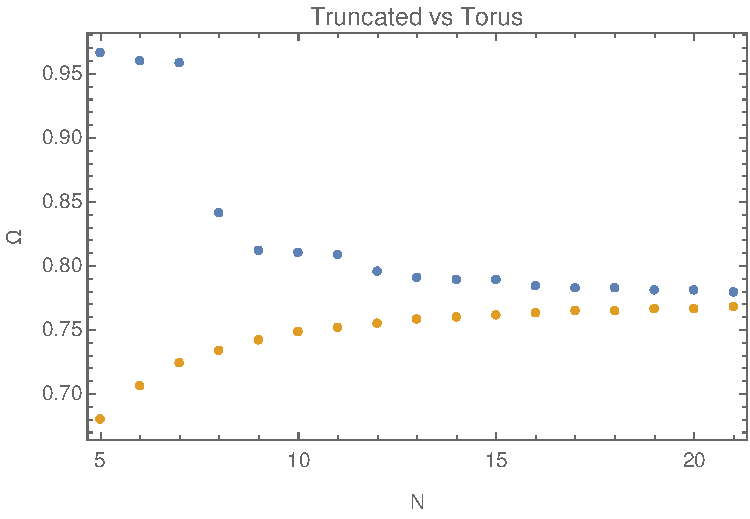
\includegraphics[width=0.6\textwidth]{p3.pdf}
	\end{center}
	\caption{The rate of convergence of a Torus vs Truncated array of resisters}
\label{fig:qual}
\end{figure}
\FloatBarrier

\subsection{Question 4}

Based on the out put of time for several values of N we find that it runs in $\mathcal{O}(n^5)$ Although it seems like it should run on $\mathcal{O}(n^3)$. Perhaps out implementation leaves something to be improved upon.

\begin{figure}[!htb]
	\begin{center}
		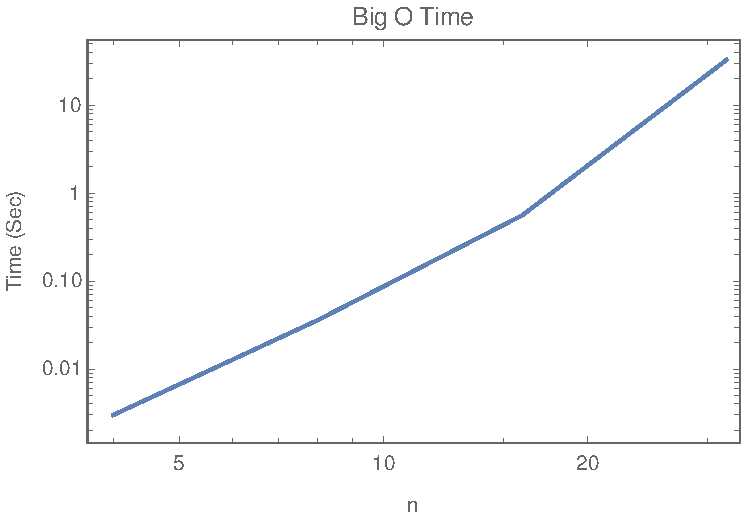
\includegraphics[width=0.6\textwidth]{p4.pdf}
	\end{center}
	\caption{The rate of convergence of a Torus vs Truncated array of resisters}
\label{fig:qual}
\end{figure}
\FloatBarrier

\section{Conclusion}

I had a really hard time developing the algorithm for turning a $N \times N$ grid into a matrix. Specifically algorithmically determining the right values for the index of the resistor and the lead to and from it. 

\end{document}

